\section{Literature review}

This literature review explores the integration of technologies in biological tissue sectioning, with a particular focus on the application of image classification and deep learning in optimizing slicing parameters. It aims to highlight significant advancements, identify gaps in current methodologies, and lay the groundwork for the proposed project.

\subsection{Microtome and Microscope}

In recent years, the advent of automatic microtomes has significantly simplified the sectioning process and improved the quality of sections.

Zimmermann, in the article "Improved reproducibility in preparing precision-cut liver tissue slices," advocates for the use of the new Leica vibratome to enhance the accuracy and reproducibility of tissue sections from rats, mice, and human tissues \cite{LR.1}.

In this experiment, the HM355S microtome provided by Epredia is used for sectioning. This machine is a popular device for biological tissue sectioning research, and many experiments and papers have utilized this equipment for sectioning.

Elzbieta Klimuszko has used the HM355S microtome for sectioning teeth to investigate the calcium and magnesium content in dental enamel \cite{LR.2}.

Andelko Hrzenjak also used the HM355S microtome for sectioning pathological endometrial tissues to study the mechanisms of endometrial carcinoma development \cite{LR.3}.

Similarly, the choice of microscope is crucial. In this experiment, the VHX7000 microscope from Keyence is used for image acquisition. It is capable of capturing images of biological tissue sections (e.g., mouse prostate cells \cite{LR.4}),
as well as inorganic materials (such as ceramics \cite{LR.5}, glass \cite{LR.6}).

The experiments will employ the HM355s microtome and VHX7000 microscope for sectioning and image acquisition. This setup ensures that both equipment selection and technological application are optimally aligned to enhance the precision and efficiency of the tissue sectioning process, supporting the overall goals of the research project.

% 近年来,自动切片机的出现显著简化了切片过程,并提高了切片的质量。

% Zimmermann在文章"Improved reproducibility in preparing precision-cut liver tissue slices"中,主张使用新的Leica振动刀来提高大鼠、小鼠和人体组织切片的精度和重复性 \cite{LR.1}。

% 在这个实验中,我们使用Epredia提供的HM355S切片机进行切片。这台机器是生物组织切片研究的流行设备,许多实验和论文都使用了这台设备进行切片。

% Elzbieta Klimuszko使用HM355S切片机切割牙齿,以研究牙釉质中的钙和镁含量 \cite{LR.2}。

% Andelko Hrzenjak也使用HM355S切片机切割病理性子宫内膜组织,以研究子宫内膜癌发展的机制 \cite{LR.3}。

% 同样,显微镜的选择也至关重要。在这个实验中,我们使用Keyence的VHX7000显微镜进行图像采集。它能够捕获生物组织切片的图像(例如,小鼠前列腺细胞 \cite{LR.4}),以及无机材料(如陶瓷 \cite{LR.5},玻璃 \cite{LR.6})。

% 实验将使用HM355s切片机和VHX7000显微镜进行切片和图像采集。这种设置确保了设备选择和技术应用的最佳配合,以提高组织切片过程的精度和效率,支持研究项目的总体目标。
\subsection{Deep Learning}

\subsubsection{Convolutional Neural Networks (CNN)}

Convolutional Neural Networks (CNNs) are a type of deep learning model that are particularly effective at processing image data. They automatically learn spatial hierarchies of features through a series of convolutional layers without the need for manual feature extraction. A typical CNN model includes layers such as convolutional layers, pooling layers, and fully connected layers \cite{DL.4}. A typical CNN architecture is shown below
:\cite{4.30 1}


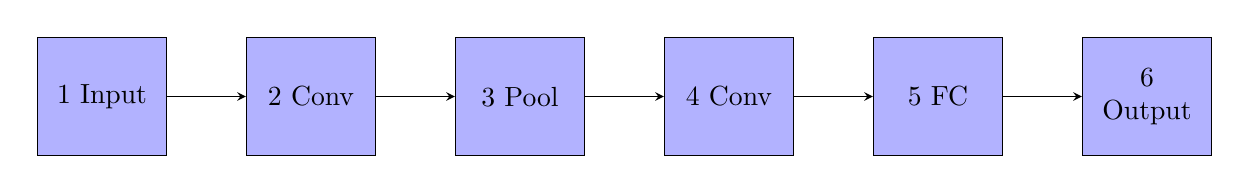
\begin{tikzpicture}[
    node distance=1cm and 0.5cm,
    block/.style={rectangle, draw, text width=4em, text centered, minimum height=15mm, fill=blue!30},
    arrow/.style={->,>=stealth}
]

% Define nodes in a matrix
\matrix [column sep=10mm, row sep=10mm] {
  \node (n1) [block] {1 Input}; & \node (n2) [block] {2 Conv}; & \node (n3) [block] {3 Pool} ;& \node
  (n4) [block] {4 Conv};    & \node (n5) [block] {5 FC};   & \node (n6) [block] {6 Output}; \\
};

% Connect nodes
\draw [arrow] (n1) -- (n2);
\draw [arrow] (n2) -- (n3);
\draw [arrow] (n3) -- (n4);
\draw [arrow] (n4) -- (n5);
\draw [arrow] (n5) -- (n6);
\end{tikzpicture}

In this model:

\textbf{Convolutional layers (Conv)}: These are the core layers of a CNN, responsible for feature extraction from images.

\textbf{Pooling layers (Pool)}: These serve to reduce the dimensionality of the feature maps, thereby decreasing the computational load.

\textbf{Fully connected layers (FC)}: These integrate the features extracted by the convolutional and pooling layers for classification or regression analysis, eventually leading to the output.

The typical method for training a CNN involves several key processes:\cite{4.30 2}

\begin{enumerate}
    \item \textbf{Forward Propagation:} Input data passes through each layer of the network until it reaches the output layer.
    \item \textbf{Loss Computation:} The network's output is compared to the actual labels using a loss function, such as cross-entropy loss, to calculate the difference.
    \item \textbf{Backpropagation:} The gradient of the loss function with respect to the network weights is computed.
    \item \textbf{Weight Update:} The network weights are updated using an optimization algorithm such as gradient descent or its variants like Adam or RMSprop, with the aim of minimizing the loss function.
\end{enumerate}

Once trained, the CNN can be employed to predict labels for new, unseen images. The distinctive feature of CNNs is their ability to automatically and efficiently learn features at different levels of abstraction, making them highly effective for tasks involving complex image data, such as medical image analysis, where accuracy and detail are paramount.\cite{4.30 3}

\subsubsection{Transfer Learning}

Indeed, for complex image tasks, constructing a simple CNN network is often insufficient. In such cases, transfer learning becomes essential. Transfer learning is a machine learning method that accelerates the training process by transferring knowledge from a pre-trained model to a new task. The core idea of transfer learning is to leverage knowledge from the source domain to aid learning in the target domain.\cite{4.30 4}

For CNN models, there are several approaches to transfer learning, such as fine-tuning and feature extraction: 

\textbf{Fine-tuning} involves adjusting the parameters of a pre-trained model to adapt it to a new task. This often includes retraining some of the convolutional layers along with the fully connected layers on the new data, which allows the model to fine-tune the features to the specific characteristics of the new dataset. \cite{4.30 5}

\textbf{Feature extraction} involves using a pre-trained model as a fixed feature extractor, where only the fully connected layers are trained on the new data. In this approach, the convolutional layers retain their learned weights and act solely to extract features, which are then used by the newly trained classifier layers to perform tasks specific to the new dataset.\cite{4.30 6}


Commonly used pre-trained models include VGG16, VGG19, Inception, and others. These models have been extensively trained on large datasets like ImageNet, where the weights of various layers in the model have been optimized and can be effectively used for transfer learning.\cite{4.30 7}

\autoref{tab:model_comparison} displays the number of parameters for models such as the VGG series (VGG16, VGG19) designed by the Visual Geometry Group at the University of Oxford \cite{DL.5}, as well as the modular deep learning models InceptionV3 \cite{DL.6} and Xception \cite{DL.7} developed by Google. These models possess a vast quantity of parameters, enabling them to accurately extract features from complex images. Utilizing the capabilities of these well-trained models allows researchers and practitioners to achieve high performance on specific tasks without the need to train the entire network from scratch, thereby saving time and resources while maintaining high accuracy.\cite{4.30 8}

\begin{table}[htbp]
    \centering
    \caption{Comparison of CNN Models}
    \label{tab:model_comparison}
    \begin{tabular}{ccccc}
        \toprule
        \textbf{Model} & \textbf{VGG16} & \textbf{VGG19} & \textbf{InceptionV3} & \textbf{Xception} \\
        \midrule
        \textbf{Number of Parameters} & 138,357,544 & 143,667,240 & 23,851,784 & 22,910,480 \\
        \bottomrule
    \end{tabular}
\end{table}

\subsubsection{Deep Learning in Tissue Sectioning}

The application of deep learning technologies in the biomedical field has achieved significant advancements. Deep learning models excel in tasks such as image classification, object detection, and segmentation, providing powerful tools for research and diagnostics in biomedical laboratories.

Lorena Guachi-Guachi proposed a method utilizing CNN networks to identify and refine tissue sections. This approach represents an innovative application of deep learning that can enhance the precision of tissue preparation and analysis \cite{LR.7}.

In the book \textit{Biomedical Texture Analysis}, Vincent Andrearczyk introduced a CNN architecture specifically designed for texture analysis, which significantly improves the accuracy of classifying biological tissues compared to traditional architectures \cite{LR.8}. This development demonstrates the potential of deep learning to enhance the detailed analysis of tissue characteristics, which is crucial for accurate diagnostics and research.

Yan Xu suggested that features extracted from CNNs trained on the large natural image database, ImageNet, can be transferred to histopathological images of tissues \cite{LR.9}. This provides a viable approach for implementing transfer learning, which can greatly enhance the efficiency of tissue image classification and analysis.

Based on the literature, deep learning technology holds broad prospects for application in image classification and analysis of tissue sections. By leveraging deep learning models, efficient identification and classification of tissue samples can be achieved, providing strong support for optimizing sectioning parameters.

This section underscores the transformative impact of deep learning on the field of tissue sectioning, promising significant improvements in the accuracy and utility of histological analyses.

% 在生物医学领域,深度学习技术的应用已取得了显著的进步。深度学习模型在图像分类、对象检测和分割等任务中表现出色,为生物医学实验室的研究和诊断提供了强大的工具。

% Lorena Guachi-Guachi 提出了一种利用 CNN 网络识别和精炼组织切片的方法。这种方法代表了深度学习的创新应用,可以提高组织准备和分析的精度 \cite{LR.7}。

% 在《生物医学纹理分析》一书中,Vincent Andrearczyk 介绍了一种专为纹理分析设计的 CNN 架构,与传统架构相比,这种架构显著提高了生物组织分类的准确性 \cite{LR.8}。这一发展展示了深度学习提高组织特性详细分析的潜力,这对于准确的诊断和研究至关重要。

% Yan Xu 提出,从在大型自然图像数据库 ImageNet 上训练的 CNN 中提取的特征可以转移到组织的病理学图像上。这为实施转移学习提供了一种可行的方法,可以大大提高组织图像分类和分析的效率 \cite{LR.9}。

% 根据文献,深度学习技术在组织切片的图像分类和分析中有广阔的应用前景。通过利用深度学习模型,可以实现组织样本的有效识别和分类,为优化切片参数提供了强大的支持。

% 这一部分强调了深度学习对组织切片领域的变革性影响,预示着在组织学分析的准确性和实用性方面的显著改进。


